%!TEX root = ../thesis.tex

\chapter{State of the Art}
\label{cha:stateofart}

In this chapter, we summarize the most relevant work on instance segmentation.
First, we focus on tracking implementations and later, we talk about the state of the art methods for instance segmentation and some implementations applied to videos.

\section{Tracking}
\label{sec:soa_tracking}

Tracking implementations are mainly focus on video object tracking.
This consists in taking the bounding box sorrounding an object and make bounding box predictions throught the video that contains the object to track.

One state of the art implementation is MDNet~\mdnet.
It proposes a Convolutional Neural Network with shared layers and multiple branches of domain-specific layers.
The architecture overview is showed at \figref{mdnet}.
Each branch is responsible for binary classification to identify the target in each specific video.
This domain-specific layers are updated online and the online tracking is performed by evaluating the candidate windows randomly sampled around the previous target state.
This showed state-of-the art results on tracking benchmarks and was the winner of the VOT Challenge~\votchallenge in 2016.

\begin{figure}[h]
  \centering
  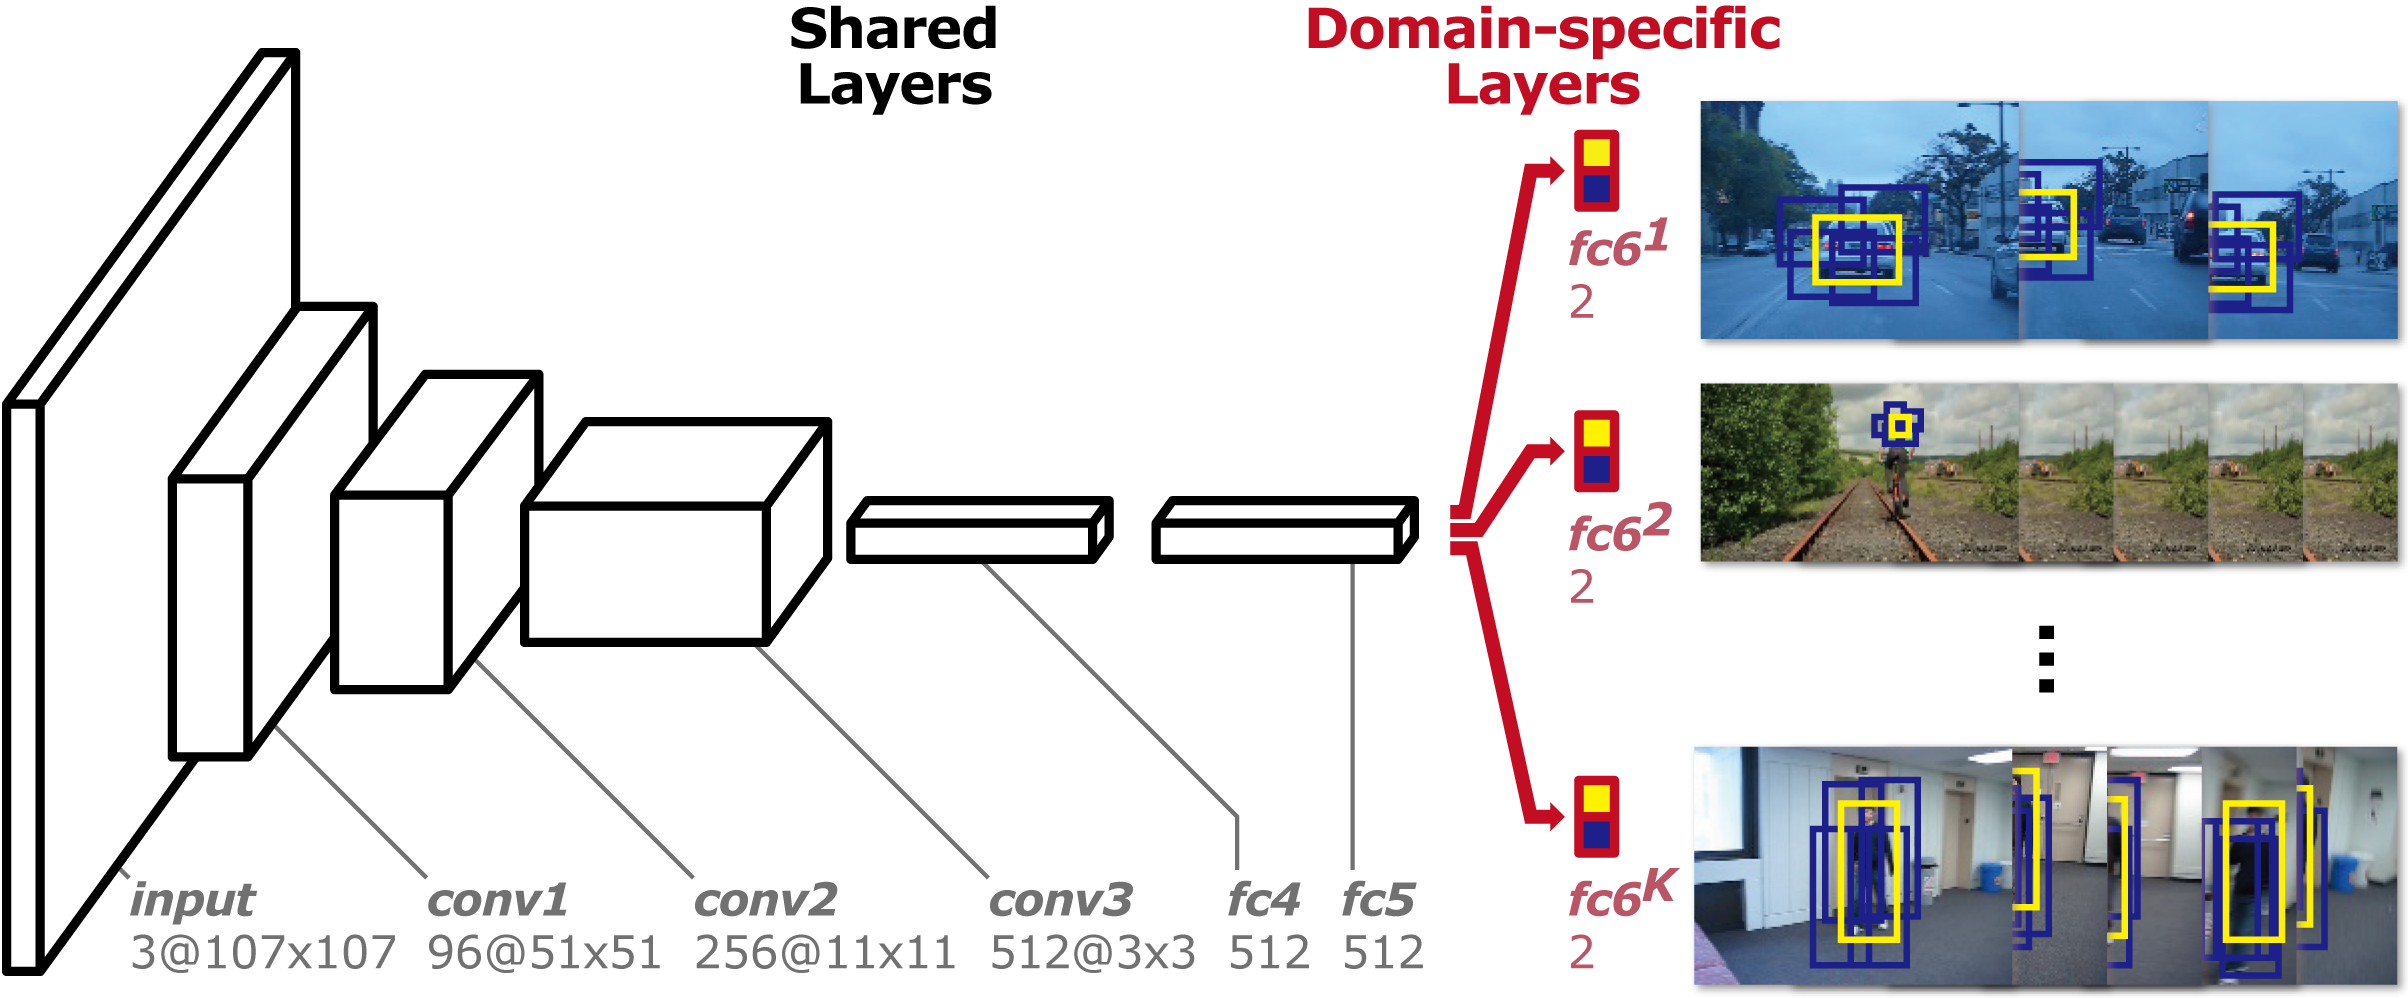
\includegraphics[width=.8\linewidth]{figures/mdnet/architecture.png}
  \caption{MDNet~\mdnet architecture. }
  \label{fig:mdnet}
\end{figure}

Unfortunetly there are not implementations that focus on keypoints tracking which is the idea behind this thesis.

% Stacked Hourglass Networks for Human Pose Estimation~\cite{newell2016stacked}


\section{Instance Segmentation}
\label{sec:soa_instancesegmentation}

Instance detection and segmentation is one of the most challenging tasks in Computer Vision right now.
In this section we explore some of the works that tackle instance segmentation in different domains like image and video.

\paragraph{Mask R-CNN~\maskrcnn}
This work come from a series of works that started with object detection on images using Convolutional Neural Networks.
Afterwards, they iterate the architecture to make it differentiable, being able to train it end-to-end.
The last iteration consisted on predicting not only the bounding box of the detected object but its mask.
The idea behind this method consists on a CNN that with a forward pass extract the features at the last convolutional layer.
Then a set of bounding box proposals are generated and the features in each proposed bounding box are used in one branch to predict a objectiveness score and bounding box regressions.
With this branch a set of bounding box are obtained and score predicted. With this values, a second branch is responsible to predict a mask from each proposal.
The final prediction use maximum supression to reduce the proposals to the final prediction masks.
This approach show state of the art results on multiple datasets at the cost of using a very large amount (in the order of 1000) proposals per a single image.
Some qualitative results can be found on \figref{maskrcnn}.

\begin{figure}[h]
  \centering
  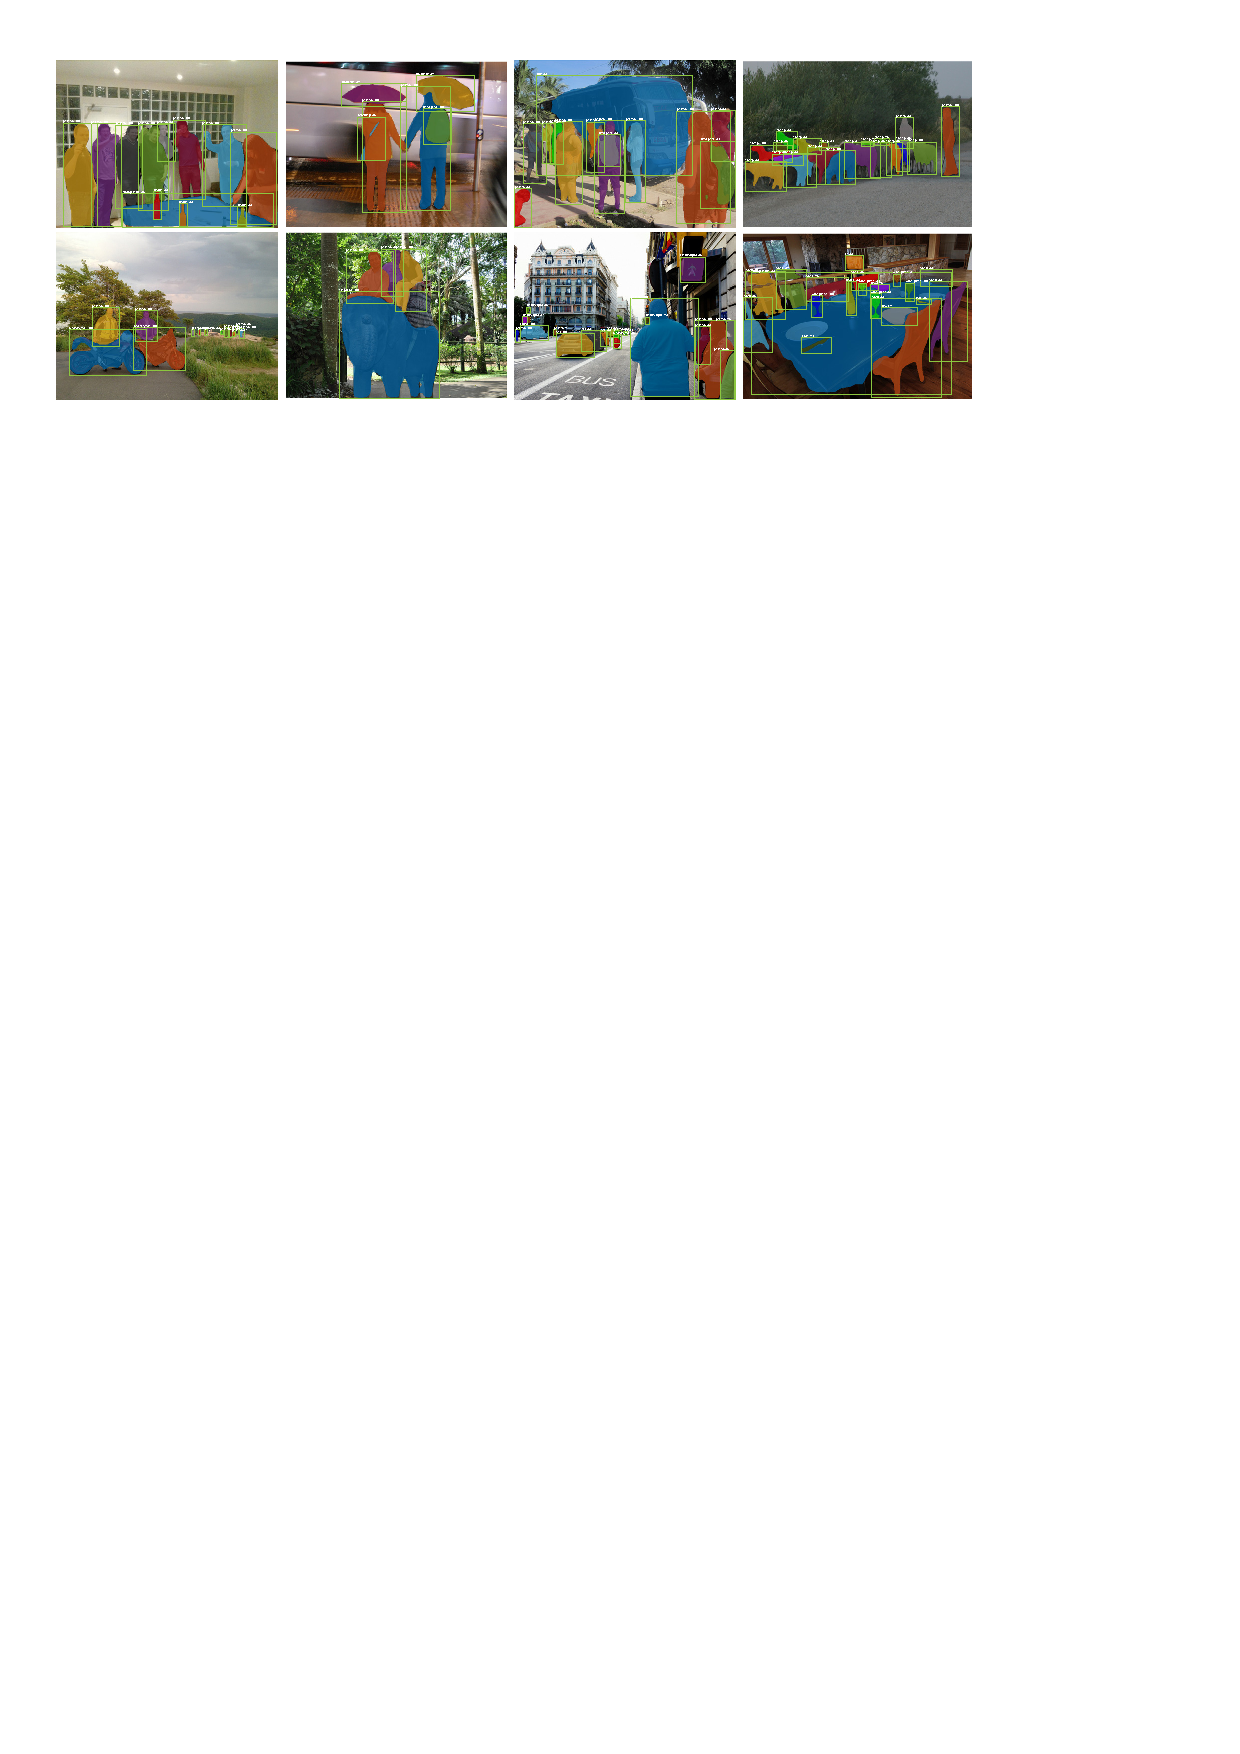
\includegraphics[width=1.\linewidth]{figures/maskrcnn/results.pdf}
  \caption{Mask R-CNN~\cite{he2017mask} results. }
  \label{fig:maskrcnn}
\end{figure}

\paragraph{Deep Metric Learning~\deepml}
This works also focus in instance object segmentation on images.
They use a Convolutional Neural Network to predict an embedding representation per each pixel.
This network is trained using metric learning, regressing how likely two pixels are to belong to the same object.
Then they propose the use of seed points and its pariwise similarity to predict the instances and its masks on an image once the embedding for each pixels is computed.
Some results of the segmentations can be found on \figref{deep_metric_learning}.

\begin{figure}[h]
  \centering
  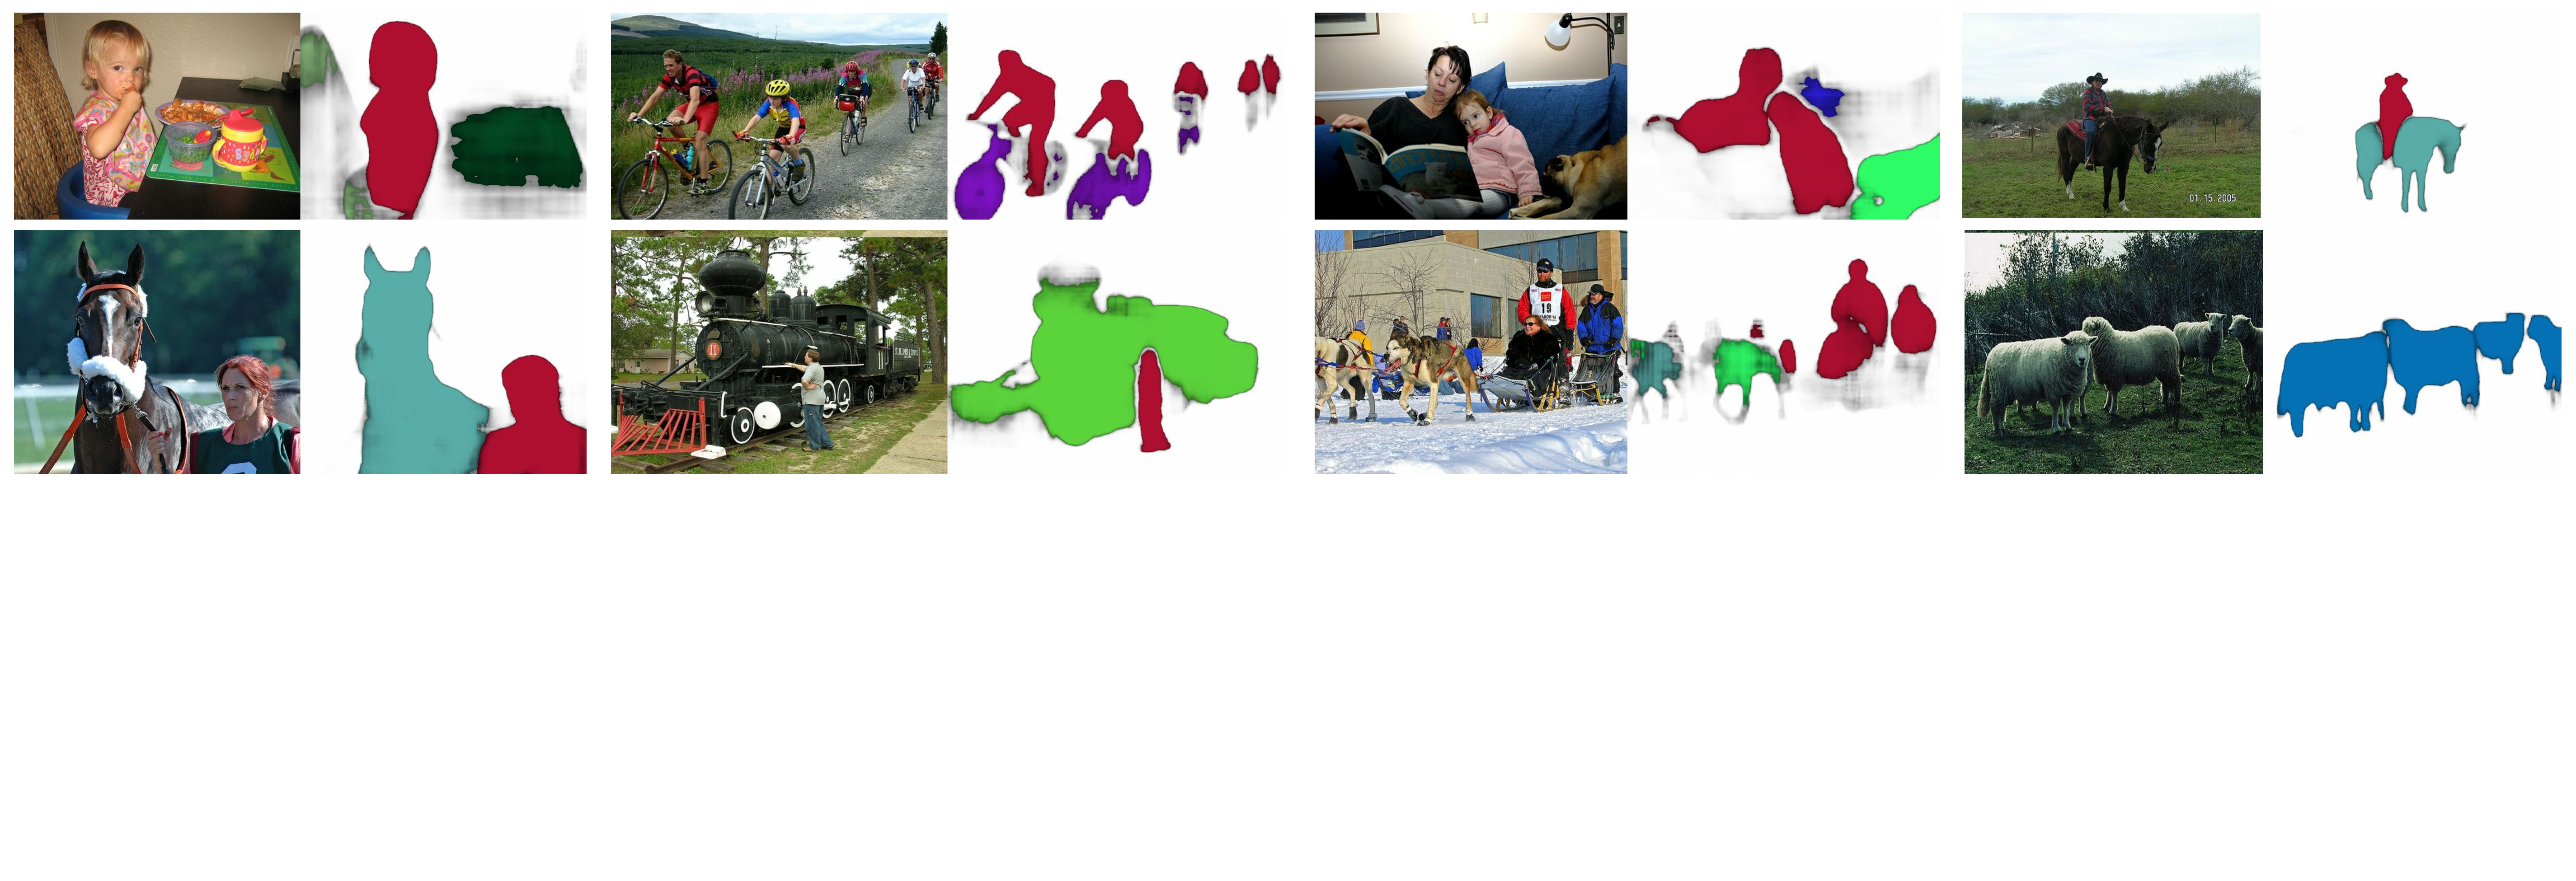
\includegraphics[width=1.\linewidth]{figures/deep_metric_learning/mask_classification.pdf}
  \caption{Deep Metric Learning~\deepml instance segmentation results. }
  \label{fig:deep_metric_learning}
\end{figure}

\paragraph{OSVOS~\osvos and OnAVOS~\onavos}
This works focus on instance segmentation on video.
Their main approach consists on train a parent network that given a frame is able to predict the mask of the foreground (all object instances in the image) and then finetune a network for each video.
This finetune is performed given the mask of the first frame (this methods tackle semi-supervised video object segmentation) and then the trained network for each video is used to predict the masks for the rest of the frames.
The OnAVOS~\onavos work in this last step add an online training.
It makes predictions of the frames and after each frame prediction, the network is online trained with the new predicted mask.
This two implementations present the state of the art results on the DAVIS~\davisboth dataset.

\paragraph{MaskRNN~\maskrnn}
This work proposes a recurrent neural network approach which fuses in each frame of the video the output of two deep nets for each objects instance.
The first net is a binary segmentation network providing a mask and the second one is a localization network providing a bounding box.
Thanks to the recurrent component and the localization component, this method is able to take advantage of long-term temporal structures of the video as well as rejecting outliers.
This method also provide competitive results with the previous works of OSVOS~\osvos and OnAVOS~\onavos.

% \paragraph{Proposal Free Network}~\cite{liang2015proposal}
